\section*{Problem 2}
	\begin{proof} [Solution]
		From the Problem 1, we have following DEs:
		\begin{align*}
			\frac{dS}{dt} &= -\beta\frac{IS}{N_0}\\
			\frac{dI}{dt} &= \beta\frac{IS}{N_0} - \gamma I\\
			\frac{dR}{dt} &= \gamma I
		\end{align*}
		Since some people in recovered group move to susceptible group, we can modify them as following:
		 \begin{align*}
		 	\frac{dS}{dt} &= -\beta\frac{IS}{N_0} + \eta R\\
		 	\frac{dI}{dt} &= \beta\frac{IS}{N_0} - \gamma I\\
		 	\frac{dR}{dt} &= \gamma I - \eta R
		 \end{align*}
	 	To check a equilibrium state, put them 0 at $S = S^*, I = I^*, R = R^*$. i.e. $S^*, I^*, R^*$ are values at equilibrium state each. Note that total population is preserved. i.e. $S^* + I^* + R^* = N_0$. Combine all 4 equations, then we get:
	 	\begin{align*}
	 		S^* &= -\frac{\gamma}{\beta}N_0\\
	 		I^* &= \frac{\eta}{\gamma + \eta}\left(1 - \frac{\gamma}{\beta}\right)N_0\\
	 		R^* &= \frac{\gamma}{\gamma + \eta}\left(1 - \frac{\gamma}{\beta}\right)N_0
	 	\end{align*}
 		This means there exists a equilibrium state for that modified DEs. But it does not lead to the end of pandemic. Because since infected population is not 0, infection and recovery are repeated. We can check it by following example plot. Here, I set $\beta = \frac{1}{3}$, i.e. $R_0 \simeq 4.667$.
 		\begin{center}
			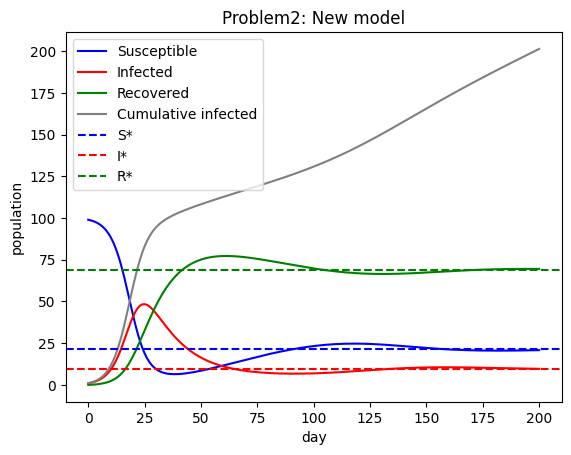
\includegraphics[scale=0.7]{Problem2_model.png}
 		\end{center}
 		Next, let analyze the trend of this model. Note that $\beta=\frac{1}{3}$, day $T = 200$. As in the below plot, $I(t)$ of model goes to 0 because there are no more people to get infected($S(t) goes to 0 also$). However, the modified model does not. Since it goes to equilibrium state, $S(t)$ and $I(t)$ are preserved after a long time.
 		\begin{center}
 			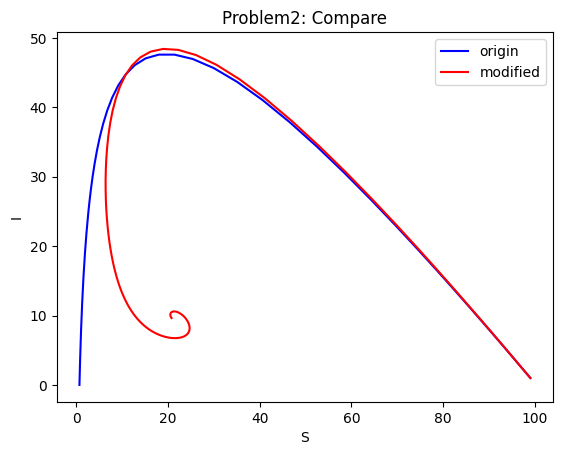
\includegraphics[scale=0.7]{Problem2_compare.png}
 		\end{center}
 		In this scenario, since the initial phase is similar to original model, proactive strategies, same as origin, may be effective. However, If the spread has begun, then we cannot fully stop the infection. In this situation, we need to continue to take care of small loops to prevent a major outbreak that will lead to pandemic again.\\
 		
	\end{proof}